% Spectroscopic methods span a wide range of regimes and objectives, including optical spectroscopy \cite{schawlow_infrared_1958}, nuclear magnetic (NMR) \cite{PhysRev.70.460,PhysRev.69.37}, electron spin resonance (ESR) and more. Among the most notable advances, \textit{Stimulated Emission Depletion} (STED) microscopy, introduced by Hell, surpasses the diffraction limit of light microscopy by selectively depleting fluorescence around a targeted nanoscale region, achieving resolutions on the order of tens of nanometers \cite{hell_breaking_1994,HELL199419}.  

% Parallel to these advancements, continuous efforts aim to overcome intrinsic spectral broadening mechanisms such as Doppler, Fourier (transit-time), and power broadening~\cite{PhysRevLett.104.053001,finkelstein_power_2019}. However, even in the absence of technical noise, the ultimate spectral resolution of a coherently driven two-level system is fundamentally limited by decoherence. According to the Bloch equations, the homogeneous linewidth scales inversely with the coherence time $T_2$, establishing the so-called $T_2$ limit~\cite{Zienau_1975,PhysRev.70.460}. While various schemes seek to mitigate this constraint through dynamical decoupling or engineered dissipation~\cite{PhysRevLett.122.060503,retzker_2,Cao_2025}, the connection between decoherence and spectral resolution is generally regarded as fundamental, as the same stochastic frequency fluctuations that govern dephasing also determine the resolvability of energy-level transitions.

% Experimentally, this limit is probed by weak-drive spectroscopy, in which a continuous tone is swept across the qubit transition while monitoring the excited-state population\cite{PhysRevLett.107.240501,PhysRevX.9.041041,spec123}. In this regime, the drive amplitude must remain sufficiently small to avoid power broadening, allowing the measured linewidth to approach the intrinsic decoherence-limited value.Increasing the drive strength enhances signal visibility but leads to transition saturation and a corresponding linewidth that grows approximately linearly with the drive amplitude. Conversely, excessively weak driving results in poor contrast and limits spectral resolvability. As a result, conventional spectroscopy operates within a narrow range of drive amplitudes that balances signal strength against power-induced broadening.

\begin{figure*}
    \centering
    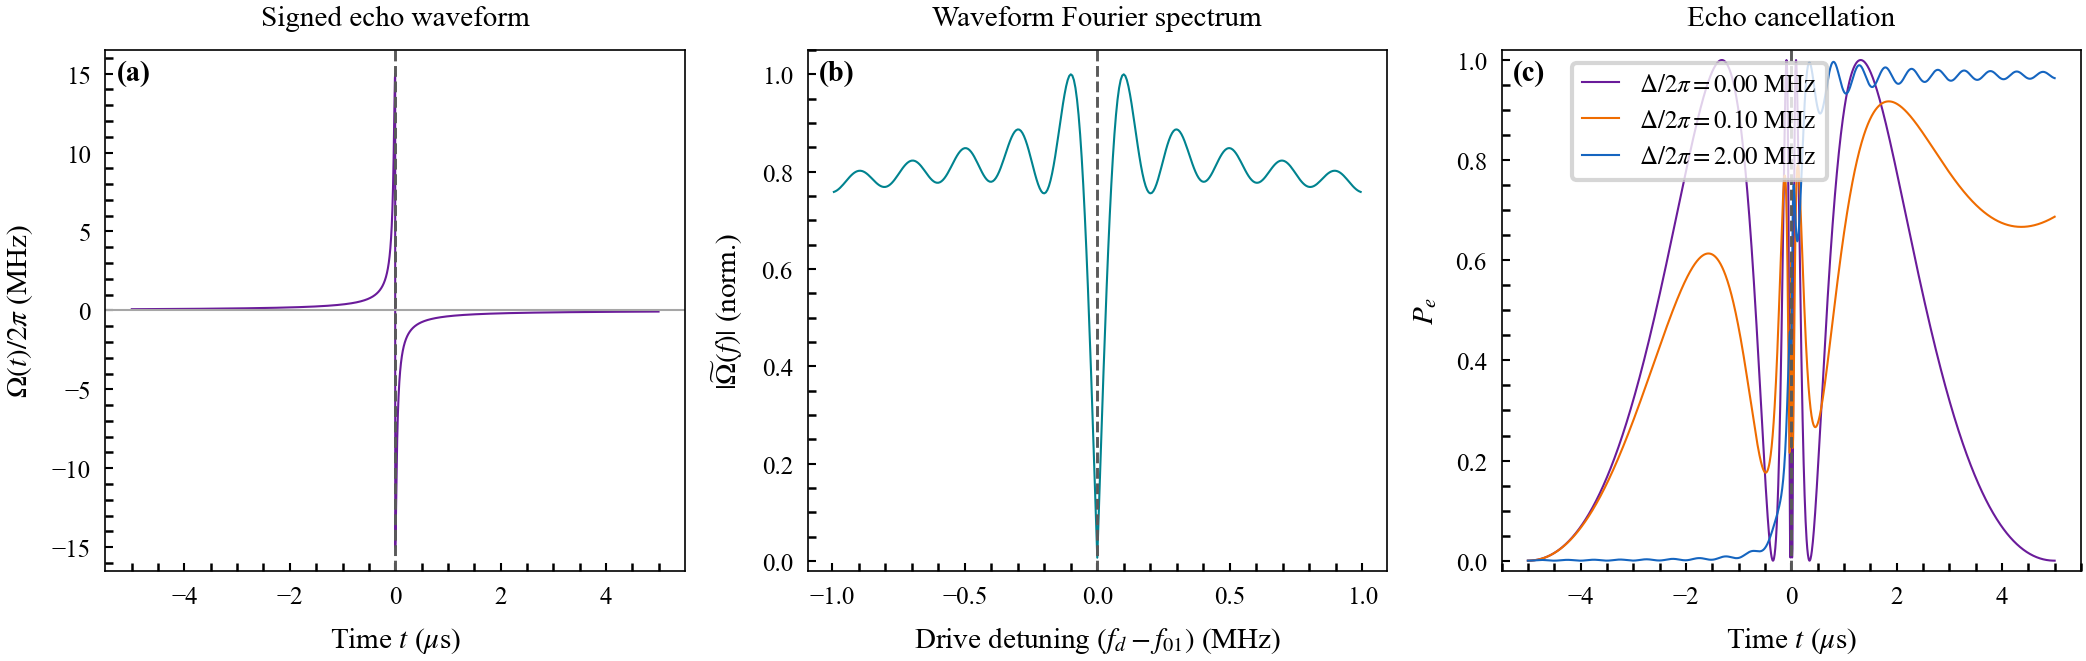
\includegraphics[width=1\linewidth]{../figures/paper/01_pulse_mechanism.png}
    \caption{
    Pulse waveform and echo-cancellation mechanism.
    (a) Signed echo-root-Lorentzian drive envelope with peak amplitude $\Omega_0/(2\pi)=15~\mathrm{MHz}$ and a $\pi$ phase inversion at the pulse midpoint.
    (b) Normalized magnitude of the waveform Fourier spectrum, showing the spectral null at zero frequency produced by the phase inversion.
    (c) Unitary two-level excited-state population during the pulse at $\Delta/(2\pi)=0$, $0.10$, and $2.00~\mathrm{MHz}$, without relaxation or dephasing. At resonance, the evolution accumulated during the first half is exactly reversed during the second half, whereas finite detuning prevents complete cancellation.}
    \label{fig:fig1}
\end{figure*}


Determining the transition frequency of a quantum system is a fundamental task
in spectroscopy, quantum metrology, and quantum sensing. The simplest setting
is a two-level system, whose energy splitting defines a spectroscopic resonance
and can encode changes in its local environment. This frequency is commonly
estimated by sweeping a coherent drive across the transition and monitoring
the resulting population response~\cite{PhysRev.70.460,PhysRev.78.695,PhysRevLett.122.060503,retzker_2}.
Such measurements underlie both the characterization of quantum devices and
the use of quantum systems as probes of external perturbations.

In direct population spectroscopy, spectral resolution and measurement
robustness are competing requirements. Conventional continuous-wave
spectroscopy generally applies a drive long enough for the population to
approach a steady state. In the weak-drive regime, decoherence produces a
homogeneous linewidth that scales as $1/T_2$, establishing the natural
coherence-limited resolution scale of the transition. Increasing the drive
strength makes the population response more pronounced, but also power broadens
the transition. Conventional high-resolution spectroscopy therefore requires
the drive amplitude to be chosen carefully, balancing a pronounced population
response against power broadening.
High-amplitude spectroscopy is further complicated when the nominal two-level
system is embedded in a multilevel spectrum. Off-resonant coupling to
neighboring transitions can produce amplitude-dependent AC-Stark shifts,
line-shape distortions, and leakage, causing the apparent resonance to move
with drive strength~\cite{PhysRevA.76.042319,motzoi_drag_2009,gambetta_analytic_2011}.






Ramsey interferometry provides a standard alternative to direct spectroscopy and, in principle, enables frequency estimation at the $T_2$ limit~\cite{PhysRev.78.695}. Other sensing protocols can surpass this probe-$T_2$ scale using inter-shot correlations, external references, dynamical decoupling, or tailored filter functions~\cite{PhysRevLett.122.060503,retzker_2,Cao_2025,gefen_clock_2016,bylander_2011,iosue_filter_2026}. Ramsey generally presupposes an approximate transition frequency and calibrated $\pi/2$ pulses for state preparation and readout, and is therefore not fully calibration independent. Achieving $T_2$-limited resolution also requires long interrogation times and sufficiently dense temporal sampling to resolve the resulting interference fringes. Finite-pulse imperfections and probe-induced frequency shifts, including unintended AC-Stark shifts during the control pulses, can nevertheless bias the extracted transition frequency~\cite{PhysRevA.98.053424,shuker_ramsey_2019}.




% In the context of superconducting circuits, circuit quantum electrodynamics (cQED) employs nonlinear harmonic oscillators—most prominently the transmon—to resolve transitions between the ground and excited states of weakly anharmonic systems. This technique, known as qubit spectroscopy, serves as a cornerstone for the calibration and characterization of superconducting quantum processors 

% Ramsey interferometry is a standard alternative to direct spectroscopy. In a typical Ramsey sequence, two $\pi/2$ pulses are separated by a free-evolution interval $\tau$, resulting in interference fringes in the excited-state population that oscillate at the detuning frequency. In practice, however, achieving $T_2$-limited spectral resolution requires both long interrogation times and sufficiently high temporal sampling to resolve the resulting oscillations. Moreover, the accuracy of Ramsey measurements is susceptible to systematic biases: asymmetries in the exponential decay envelope—arising, for example, from pulse miscalibration—can shift the perceived resonance peak in the frequency domain. Additional effects such as phase fluctuations or unintended AC-Stark shifts during the control pulses introduce further distortions, ultimately biasing the extracted frequency estimate.\cite{PhysRevA.98.053424,PhysRev.78.695,wang_coherent_2019}.
